%\documentclass{jarticle}
%\newcommand{\figref}[1]{\figurename\ref{#1}}
%\newcommand{\tabref}[1]{\tablename\ref{#1}}
%\usepackage[dvipdfmx]{graphicx}
%\begin{document}

%\section{解析}
\subsection{エネルギー解析}
信号解析で求めたエネルギーの値を元にミッシェルパラメータを求めるための各種解析を行った.
まずは時間情報を元にスピンの向きに関する考察をし,さらにバックグラウンドの影響を考えてイベントのセレクションを行った.
また,エネルギースペクトルに対するフィッティングでは検出器内での電磁シャワーによるエネルギー応答を考慮して行列を関数に畳み込んで最小二乗法を適用した.

\subsubsection{スピンの回転に関して}
当初の計画とは異なるが$g$ 因子測定用の磁場標的データを用いて以下の解析を行った.
このデータを元に解析を行ってもミッシェルパラメータの測定ができることがわかったため,長い時間の測定データを使う方が統計誤差の観点から良いためである.
また,このデータはスピン方向の情報を持っているため,スピンに関わるミッシェルパラメータである$\xi,\delta$ の測定も可能である.
以下ではまず時間情報を元にスピン方向が求められる事をみる.

崩壊時間の分布は$g$ 因子の解析で説明したように減衰部分と振動部分の積の形で出てくる.
$\rho$ を求めるためには無偏極のデータを得る必要があるが,スピン歳差運動の一周期分の時間範囲のデータを取り出しても,指数の減衰があるためスピン方向を等価に足しあわせることができない.
そこで,減衰の逆数で重みをつけることを考える.
ここではミューオンの崩壊寿命$\tau=2.2~\mathrm{\mu s}$ を既知として各イベントについて$\exp(t/\tau)$の重み付けを行った.
すると崩壊時間重みつき分布は\figref{hatano_fig:oscillation} のようになった.
これは実際に指数関数の影響をキャンセルしてスピンに由来する情報のみを取り出せてることを示している.

\begin{figure}[hbt]
\centering
\includegraphics[width=0.6\textwidth]{figure/hatano/oscillation_modify1.eps}
\caption{時間に対するスピンによる計数の変動の様子.指数関数の逆数で重みをつけた.}
\label{hatano_fig:oscillation}
\end{figure}

以上より,同様の重み付けをした上で適切な時間範囲をとることで,任意のスピンの向きに関するエネルギースペクトルを取り出すことができる.

\subsubsection{イベントセレクション}
標的方向からの粒子はフィンガーカウンターが鳴っているという条件を課すと中心のNaI に大部分のエネルギーを落とすと考えられるので,バックグラウンドを減らすために中心のNaI と全体とのエネルギー比$\alpha$ を用いてイベントセレクションを行った.
比の値$\alpha$ について,$\alpha=0,0.2,0.4,0.6,0.8,1.0$ 以上のイベントを選んだ時のエネルギースペクトラムを\figref{hatano_fig:bg} に示す.
$\alpha=0.2,0.4,0.6,0.8$ ではイベント数が減るだけで分布の相対的な形は大きな変化をせず,以降の解析の値に大きな変化はなかった.
以下の解析では,$0.2\leq\alpha\leq0.8$ の範囲でミッシェルパラメータ$\rho$ のフィッティングの$\chi^2$ が最小となった$\alpha=0.6$ とした.
\begin{figure}[hbt]
\centering
\includegraphics[width=0.6\textwidth]{figure/hatano/bg_modify1.eps}
\caption{NaI で測定した$e^+$ のエネルギー分布.中心のNaI と全体のNaI とのエネルギー比を用いてカットを行ったときの変動を示す.}
\label{hatano_fig:bg}
\end{figure}

\subsubsection{検出器の電磁シャワー応答について}
今回の検出器はNaI結晶による全吸収型のカロリメータではあるが,検出器内で形成された電磁シャワーで主に$\gamma$ 線となったものが検出器内から漏れる事が多いため,必ずしも入射した粒子のエネルギーに比例したエネルギーが測定されるわけではなく,低エネルギーの裾をもつ分布になる.
ただし,この関数形を解析的な形で求めることは難しいので今回はGeant4 を用いたシミュレーションを行って,応答を計算した.
結果を\figref{hatano_fig:response}に示す.
観測するエネルギーは入射した$e^+$ のエネルギー付近にピークを持ち低ネルギーの裾を持つ分布になっていることが分かる.
観測するエネルギーが入射したエネルギーよりも高くなるのは,検出器中の$e^-$ との対消滅によるものと考えられる.

\begin{figure}[hbt]
\centering
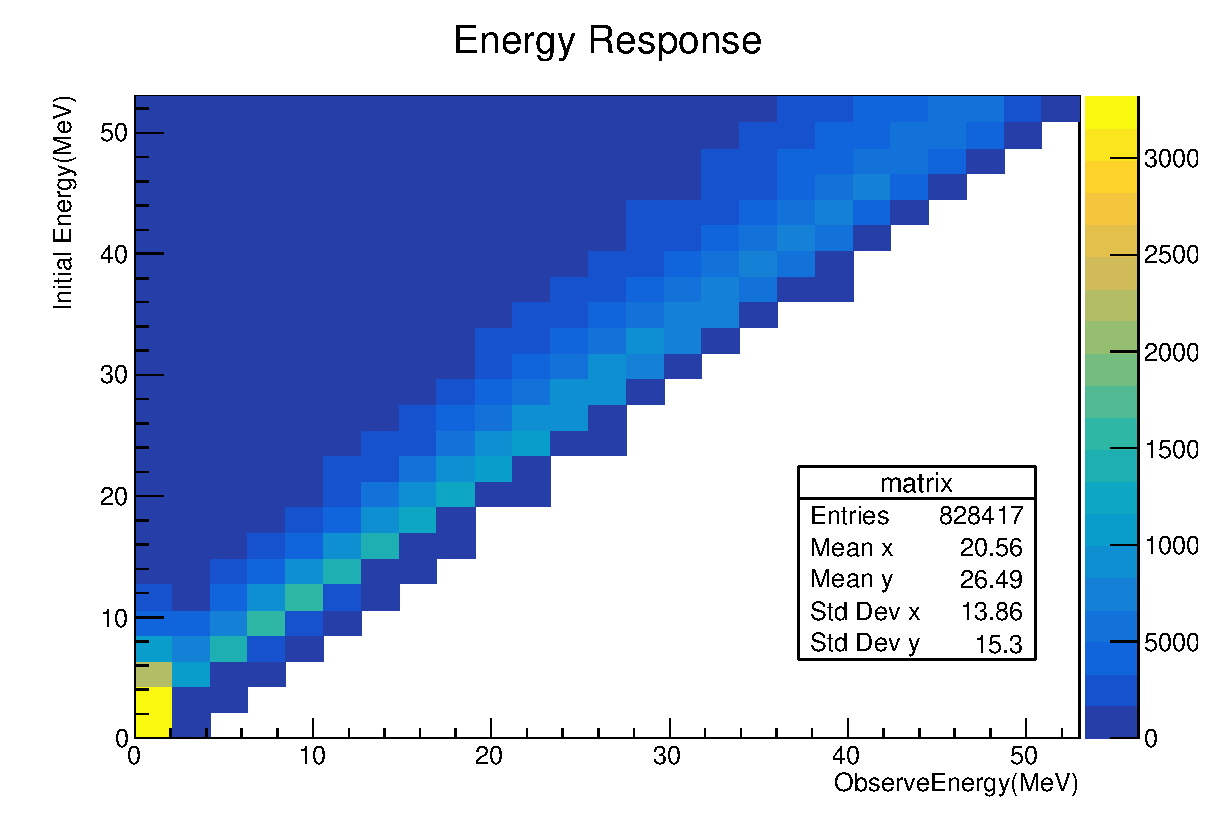
\includegraphics[width=0.6\textwidth]{figure/hatano/response.eps}
\caption{検出器内の電磁シャワー応答のシミュレーション.縦軸は検出器に入射した$e^+$ のエネルギー,横軸は検出器で観測した$e^+$ のエネルギーを示す.}
\label{hatano_fig:response}
\end{figure}

以下の解析ではこの応答を畳み込んだ最小二乗法を用いた.
最小二乗法の詳細については付録Bに掲載する.

\subsubsection{ミッシェルパラメータ$\rho$ の導出}
スピンが無偏極のときのエネルギースペクトルは\eqref{hatano_eq:rho}と表される.
ここでは,無偏極データを得るために\figref{hatano_fig:oscillation}の最初の三周期に相当する範囲を抽出した.
この際,各イベントには指数関数の逆数で重みをつけた.
\begin{equation}
  f(x)=(3 - 3x / E_\mathrm{max})+\frac{2}{3}\rho(4x / E_\mathrm{max} - 3)
  \label{hatano_eq:rho}
\end{equation}
このデータに対して,\eqref{hatano_eq:rho}の関数でフィッティングを行うわけだが,このフィッティングは高エネルギー部分の分布に敏感であり,そのため較正係数の誤差の影響が大きい.
較正計数を測定誤差である$\pm 20~\%$ の範囲で動かし,$\chi^2$ が最小になったときを測定値とした.

フィッティングの結果を\figref{hatano_fig:rho} に示す.(バックグラウンドとして一次関数を仮定した).
この時のフィッティングのパラメータは$f(x)$を$p_0(3 - 3x / E_\mathrm{max}) + \frac{2}{3} p_{1} (4x / E_\mathrm{max} - 3)$ ,バックグラウンドを$p_2+p_3x$ と書くと,\tabref{hatano_tab:rho} に示す値になった.
これより,ミッシェルパラメータ$\rho$は$\rho=0.662 \pm 0.022$ と求まった.

\begin{table}[hbt]
\centering
\caption{$\rho$ のフィッティングパラメータ}
\begin{tabular}{cc|cc|cc|cc}
$p_0$ & $\delta p_0$ & $p_1$ & $\delta p_1$ & $p_2$ & $\delta p_2$ & $p_3$ & $\delta p_3$ \\ \hline
3.092 & 0.011 & 4.665 & 0.128 & 1476.440 & 0.158 & -2.660 & 0.011
\end{tabular}
\label{hatano_tab:rho}
\end{table}

最小二乗法ではフィッティングパラメータの推定値から$1\sigma$ ずれた時に$\chi^2$ の値は$chi^2_{min}+1$ となる.\cite{leo} 
較正からの系統誤差を求めるために,較正較正を動かし$\chi^{2}_{min} + 1$ 以下であるところを求めた.
最大で0.801,最小で0.617 であり$\rho=0.662$ との大きい方の差である0.138 を系統誤差とした.
以上の結果をまとめると$\rho=0.662 \pm 0.022 (stat.) \pm 0.138 (syst.)$ である.

\begin{figure}[hbt]
\centering
\includegraphics[width=0.6\textwidth]{figure/hatano/rho_modify1.eps}
\caption{$\rho$ のフィッティングの様子.黒点で示したのが測定値,赤線がフィッティングした曲線.}
\label{hatano_fig:rho}
\end{figure}

\subsubsection{ミッシェルパラメータ$\xi$ の導出}
式\eqref{eq:theory_michel} をエネルギーで積分すると,式\eqref{hatano_eq:xi} となる.これはスピンの向きに対する計数率の変化を表す.

\begin{equation}
  \frac{dN}{d\cos\theta} \propto \int^1_0 x^2dx\left[ (3-3x) + \frac{2}{3}\rho(4x-3) + \xi\cos\theta\left\{ (1-x) + \frac{2}{3}\delta(4x-3) \right\}\right] = \frac{1}{4} + \frac{1}{12}\xi\cos\theta
  \label{hatano_eq:xi}
\end{equation}

計数についてスピンが正偏極($0\leq\theta\leq\frac{\pi}{2}$) の時を$N_+$ ,負偏極($\frac{\pi}{2}\leq\theta\leq\pi$) の時を$N_-$ とし計数の比を$R=\frac{N_+}{N_-}$ と定義する.
式\eqref{hatano_eq:xi} を$\theta$について積分すると式\eqref{hatano_eq:xi_plus},\eqref{hatano_eq:xi_minus},\eqref{hatano_eq:xi_R} となる.
\begin{eqnarray}
  N_+ & \propto & \int^0_1 d(\cos\theta) \left(\frac{1}{4} + \frac{1}{12}\xi\cos\theta\right)=-\frac{1}{4}-\frac{1}{24}\xi \label{hatano_eq:xi_plus} \\
  N_- & \propto & \int^{-1}_0 d(\cos\theta) \left(\frac{1}{4} + \frac{1}{12}\xi\cos\theta\right)=-\frac{1}{4}+\frac{1}{24}\xi \label{hatano_eq:xi_minus} \\
  R  & = & \frac{6+\xi}{6-\xi} \label{hatano_eq:xi_R}
\end{eqnarray}

これはスピンの向きに関する部分の測定なので,単純なバックグラウンドだけでなくターゲット内散乱により無偏極となったものによるバックグラウンドも考えなければならない.
特に後者の影響を見積もる事は難しいが,どちらも$\xi$ を小さく見積もる方向に影響を与える.

最初の一周期の該当する範囲で重みを付けた計数は$N_+=73607.5$,$N_-=52878.6$ となる.
式\label{hatano_eq:xi_ratio} を$\xi$ について解くと$\xi=6(R-1) / (R+1)$ となり,これより$\xi=0.983\pm0.017 (stat.)$ となる.

\subsubsection{ミッシェルパラメータ$\delta$ の導出}
式\eqref{eq:theory_michel} よりスピンが正偏極の時から負偏極の時のエネルギースペクトラムを引くと,式\eqref{hatano_eq:delta} となる.ただし,この時スピンの偏極の割合は同じものとする.
この式よりミッシェルパラメータ$\delta$ を決定することができる.
\begin{equation}
  \frac{d\Gamma}{x^2dx} \propto 2 \int d(\cos\theta) \xi \left[ (1-x) + \frac{2}{3}\delta(4x-3) \right] \propto (1-x) + \frac{2}{3}\delta(4x-3)
  \label{hatano_eq:delta}
\end{equation}


正偏極のデータは$0\leq\theta\leq\frac{\pi}{2}$ を負偏極のデータは$\frac{\pi}{2}\leq\theta\leq\pi$ の最初の二周期の該当する範囲で重みをつけたエネルギースペクトラムを用いた.
正偏極のデータから負偏極のデータを差し引いたエネルギースペクトルに対して$\rho$ の解析と同様にフィッティングを行った.
その様子が\figref{hatano_fig:delta} である.
フィッティングのパラメータは\eqref{hatano_eq:delta} を$p_0(1-x/E_{max})+p_1\frac{2}{3}(4x/E_{max}-3)$ ,バックグラウンドを$p_2+p_3x$ と書くと\tabref{hatano_tab:delta} となった.
これよりミッシェルパラメータ$\delta$ は$\delta=0.641\pm0.117$ と求まった.
系統誤差も$\rho$ と同様に行うと最小で0.464,最大で0.794 となったので,大きい方の差の0.197 を系統誤差とした.
以上の結果より$\delta=0.641\pm0.117 (stat.) \pm0.197 (syst.)$ である.

\begin{table}[hbt]
\centering
\caption{$\delta$のフィッティングパラメータ}
\begin{tabular}{cccccccc}
$p_0$ & $\delta p_0$ & $p_1$ & $\delta p_1$ & $p_2$ & $\delta p_2$ & $p_3$ & $\delta p_3$ \\ \hline
0.978 & 0.123 & 1.595 & 0.211 & 104.741 & 2.722 & 0.211 & 0.123 \\
\end{tabular}
\label{hatano_tab:delta}
\end{table}

\begin{figure}[hbt]
\centering
\includegraphics[width=0.6\textwidth]{figure/hatano/delta_modify1.eps}
\caption{$\delta$ のフィッティングの様子.黒点で示したのが測定値,青線がフィッティングした曲線.}
\label{hatano_fig:delta}
\end{figure}

%\end{document}
